\chapter{Background}\label{chap:background}

This chapter introduces the theoretical background for our heuristics. We first introduce the background of planning and heuristics, and then define a formal framework for planning which will be used for the remainder of this paper. We then introduce and provide a framework for Integer Linear Programs, explaining how they can be used to solve relaxed POCL planning problems for heuristic estimates.\\


\section{Planning and Heuristics}


\textit{Planning} describes a class of problems and associated solvers which search the space of \textit{world models} to get from a given starting world model to a world model fitting given goal criteria. For any world model a set of applicable actions exists, each of which is a transformation to a new world model. By exploring the search space through actions, a \textit{planner} can find sequences of actions which lead to the goal. We specifically consider \textit{Propositional STRIPS} planning. \textit{Propositional} means that each variable is a proposition, signifying it can only be true or false, and all formulas are \textit{grounded}, denoting that they comprise solely of propositions and logical connectives. \textit{STRIPS} is a planning notation defined by~\cite{Fikes1971STRIPS}. There are multiple sub-classes of planning, which can have different definitions of world models and different methods of exploring their search space. One of these sub-classes is \textit{state-based} planning, where a world model is represented by the set of propositions and their values, called a \textit{state}, along with a sequence of actions which lead from the initial state to the current state. Another sub-class is \textit{Partial Order Causal Link} (POCL) planning, where each world model is its own \textit{partial plan}. These partial plans contain action instances called \textit{steps}, orderings between those steps, and causal links representing causal relationships between effects and preconditions of different steps.\\


The problem of \textit{PLANSAT}, determining whether a planning problem instance is solvable, and \textit{PLANMIN}, determining whether there is a solution using at most $n$ action, are both PSPACE-complete in Propositional STRIPS planning without severe restrictions, as found by~\cite{Bylander1994ComplexityOfSTRIPS}. Note that in partial-order planning, instead of PLANMIN, it is often more relevant to find whether there is a solution in at most $n$ time steps, in order to take advantage of parallel action execution. The number of time steps a solution takes is called its \textit{makespan}. To solve these intractable problem classes, \textit{heuristics} are used to generate estimates of solution length when using the current world model. As these heuristics usually need to be calculated for an exponentially growing set of search nodes, efficiency is critical, and so almost all planning heuristics run in polytime. In addition to efficiency, there are other metrics that are important to consider for heuristic effectiveness. \textit{Admissible} heuristics never overestimate the number of actions required to meet the goal, guaranteeing optimality of the first found solution when expanding nodes in order of current actions used + heuristic estimate. An admissible heuristic $H_1$ \textit{dominates} another admissible heuristic $H_2$ if for any search node $x$, $H_1(x)>H_2(x)$, since this means that it creates more accurate estimates, dominant heuristics are considered more powerful. An \textit{informed} heuristic takes into consideration problem specific information or current search progress in its calculations. We say that a heuristic is \textit{more informed} than another if it uses more of the situational information available to it within its calculations.\\


In this paper, we are particularly looking into the use of heuristics for determining PLANSAT in POCL planning. While technically this problem is PSPACE-complete, as with almost all PLANSAT problems,~\cite{Balcazar1996ImplicitGraphs} explains how `the standard complexity classes of complexity theory do not allow for direct classification of most of the problems solved by heuristic search algorithms' due to the lack of consideration for implicit inputs within the node expansion procedure, for example node size as a heuristic input. In POCL planning, node sizes are significantly larger than node sizes in state-based planning, as they contain orderings and causal links, and this increases the complexity of heuristics.~\cite{Bercher2021POCLComplexities} shows that a standard delete-relaxation heuristic in state-based planning, which is in P, becomes NP-complete when translated to POCL planning. This added complexity means that most POCL heuristics throw away information from the current search node to allow for a polytime heuristic, but this leads to an inefficient search process as current search progress is ignored when calculating future search direction. We define an NP-complete heuristic which maintains all node information, and is hence a more accurate and informed translation of state-based planning heuristics. The benefit of large node sizes in POCL planning is that a single node represents up to a factorial number of action sequences, whereas a state-based planning node only represents one. This means that calculating infeasibilty of a planning problem in POCL planning could have a significant advantage over state-based planning in some problem classes, as a single NP-complete time cut in POCL may require a factorial number of polytime cuts in state-based planning.


\section{Formalisation of Propositional STRIPS Planning}

Here we provide the formal framework for planning which will be used for the remainder of this paper. We consider the problem of determining solvability and minimal makespan for partially ordered plans. We first define a classical planning problem and plan in STRIPS notation, and then extend it to POCL problems and plans. We follow the notation used by~\cite{Bercher2020POPvsPOCL}.\\


A \textit{classical planning problem} $\mathcal{P}$ is given by a tuple $(V,A,s_I,g)$, where $V$ is a finite set of propositional state variables, $A$ is a finite set of \textit{actions}, $s_I\in 2^V$ is the initial state, and $g\subseteq V$ is the goal description. An \textit{action} $a\in A$ is a tuple $(\Pre, \Add, \Del)$; referred to as $\Pre(a)$, $\Add(a)$, and $\Del(a)$; where $\Pre, \Add, \Del \subseteq V$. These sets represent an action's \textit{precondition}, \textit{add}, and \textit{delete} lists. The precondition list holds the propositions required to execute an action, and so $a\in A$ is executable in a state $s\in 2^V$ if and only if $\Pre(a)\subseteq s$. The add list holds the propositions that will be set to true after an action is executed, and the delete lists similarly holds the propositions which will be set to false. From this, if $a$ is executable in $s$, we can define a state transition function $\gamma : A \times 2^V \rightarrow 2^V$ to return the successor state after executing $a$ in $s$: $\gamma (a,s)=(s\setminus \Del(a))\cup \Add(a)$. A sequence of actions $\overline{a}=(a_0,a_1,\ldots,a_n)$ is executable in a state $s_0$ if there exists a state sequence $\overline{s}=(s_1,s_2,\ldots ,s_{n+1})$ such that each successive action in $\overline{a}$ transitions to the next state in $\overline{s}$, or formally that $\gamma (a_{i-1},s{i-1})=s_i$ holds for all $1\leq i \leq n+1$. The state $s_{n+1}$ is called the \textit{result} of executing the sequence. If a state $s\in 2^V$ is such that $g\subseteq s$ then it is called a \textit{goal state}.\\


Classical solutions to planning problems are called \textit{total-order} plans, since they are defined with action sequences which follow a sequential order, as defined below. Figure~\ref{fig:totalOrder} shows an example of a total-order plan.

\begin{definition}
    An action sequence $\overline{a}$ is called a \textit{total-order plan} $\overline{P}$ (also \textit{total-order solution}) for a classical planning problem if and only if it is executable in $s_I$ and results in a goal state.
\end{definition}


\begin{figure}[th!]
    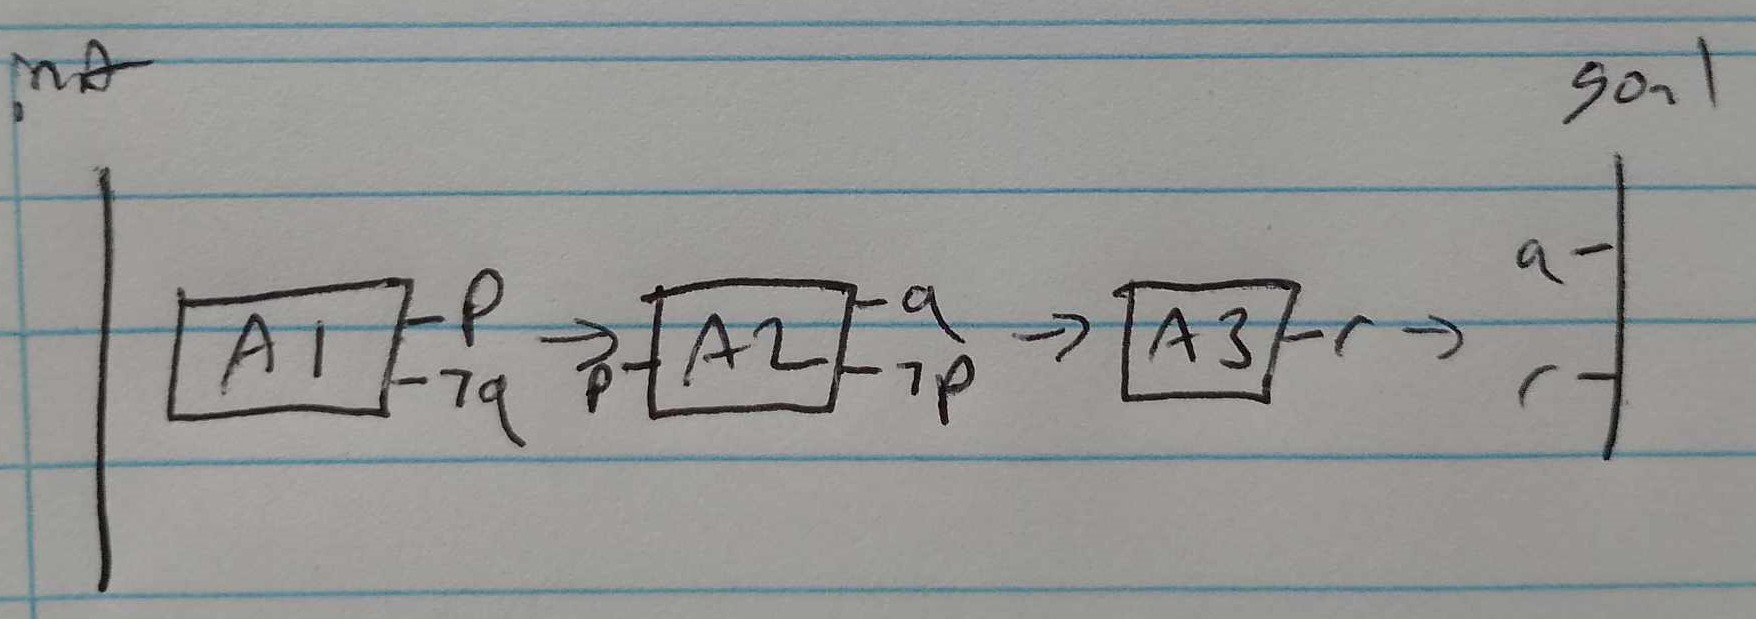
\includegraphics[width=12cm]{figures/total_order.jpg}
    \caption{An example of a total-order plan.\label{fig:totalOrder}}
\end{figure}


For the creation of our heuristic, we emulate the delete relaxation heuristics of state-based total-order planning. These heuristics utilise the delete relaxation of classical planning problems. In state-based planning, a search node represents a state, and so by substituting $s_I$ for the state of the current search node, a new classical planning problem can be created, and the solution length of its delete relaxation can be used as a heuristic value. Hence, it is important to more formally define the delete relaxation of a classical problem..\\


The \textit{delete relaxation} of a classical planning problem $\mathcal{P}$ is the problem $\mathcal{P}^+$, which is $\mathcal{P}$ but with $\Del(a)=\emptyset$ for all $a\in A$, meaning that all delete effects of actions are removed. By ignoring all delete effects in future actions, any action that becomes executable will forever remain executable.

\begin{definition}
    An action sequence $\overline{a}$ is called a \textit{relaxed total-order plan} $\overline{P}$ (also \textit{relaxed total-order solution}) for a classical planning problem $\mathcal{P}$ if and only if $\overline{a}$ is a total-order plan for $\mathcal{P}^+$.
\end{definition}


We will next extend this definition to POCL plans. POCL planning does not produce total-order plans, and instead relies on \textit{orderings} and \textit{causal links} to produce \textit{partially ordered} plans with up to a factorial number of \textit{linearizations}: total-order plans which meet the ordering and causality criteria of the POCL plan. When using POCL search algorithms to solve planning problems, search nodes are \textit{partial plans}, as opposed to classical planning where each search node is a \textit{state}. We will also refer to these partial plans as \textit{plans} for short when it is clear from context that we are referring to a partial plan and not a solution.\\


A \textit{partial plan} $P$ is given by a tuple $(PS,\prec , CL)$, where $PS$ is a finite set of \textit{plan steps}, $ps=(l,a)$, with $l$ being a unique label and $a\in A$ being an action, $\prec$ is a \textit{partial order} on $PS$, and $CL$ is a finite set of \textit{causal links}. Plan steps require unique labels to differentiate between multiple occurrences of the same action within a partial plan. As with actions, we use $\Pre(ps),\Add(ps),$ and $\Del(ps)$ to refer to the precondition, add, and delete lists of a plan step's action. A partial order is a finite set of orderings between steps, where $ps_n \prec ps_m$ represents that the step $n$ must precede the step $m$ in any linearization of the plan. A causal link is used to formally represent a causal dependency between plan steps, and is given by a tuple $(ps_p, v, ps_c)\in CL$ where $ps_p \in PS, v\in V, ps_c \in PS$. This causal link specifies how the precondition $v$ of the \textit{consumer} plan step $ps_c$ is being met, by indicating that it is \textit{supported} by the add effect $v$ of the \textit{producer} plan step $ps_p$. This means that any potential for the add effect $v$ to be deleted before the consumer step $ps_c$ requires it is a threat to the executability of $ps_c$. Such a situation, where a plan step $ps_t$ with $v\in \Del(ps_t)$ may be ordered between $ps_p$ and $ps_c$ is called a \textit{causal threat}, and $ps_t$ is called a \textit{threatening} plan step. This causal threat can be \textit{resolved} by ensuring that the threatening step $ps_t$ is either ordered before $ps_p$, or after $ps_c$, by adding an ordering constraint. Due to the requirement to resolve all causal threats, the variable $v$ is said to be \textit{protected} by its causal link as any causal threat to this protection is raised as a \textit{flaw} in the plan. We always assume for simplicity and without loss of generality that there is an implicit ordering constraint $ps_p\prec ps_c$ created for each causal link.\\

In POCL planning, the problem's initial state and goal description are encoded using two artificial actions, labelled $\mathit{init}$ and $\mathit{goal}$, where $\Add(\mathit{init})=\{v\in s_I: v \text{ is true}\}$, and $\Pre(\mathit{goal})=g$. The sets $\Pre(\mathit{init}),\Del(\mathit{init}),\Add(\mathit{goal}),$ and $\Del(\mathit{goal})$ are all empty. In all partial plans, $\mathit{init}$ is ordered before all other steps and $\mathit{goal}$ is ordered after them. This ensures that the only role of $\mathit{init}$ is to establish all initial propositions at the beginning of the plan, and the only role of $\mathit{goal}$ is to ensure that the goal description is met at the end of the plan. Having these artificial actions allows all reasoning to be done with actions, removing all state-based logic from POCL planning.\\


We can now define POCL solutions to classical planning problems. Figure~\ref{fig:partialOrder} shows an example of a POCL plan, for which the total-order plan from Figure~\ref{fig:totalOrder} is a linearization.

\begin{definition}
    A partial POCL plan $P$ is called a \textit{POCL plan} (also \textit{POCL solution}) for a classical planning problem if and only if every precondition is supported by a causal link and there are no causal threats.
\end{definition}


\begin{figure}[th!]
    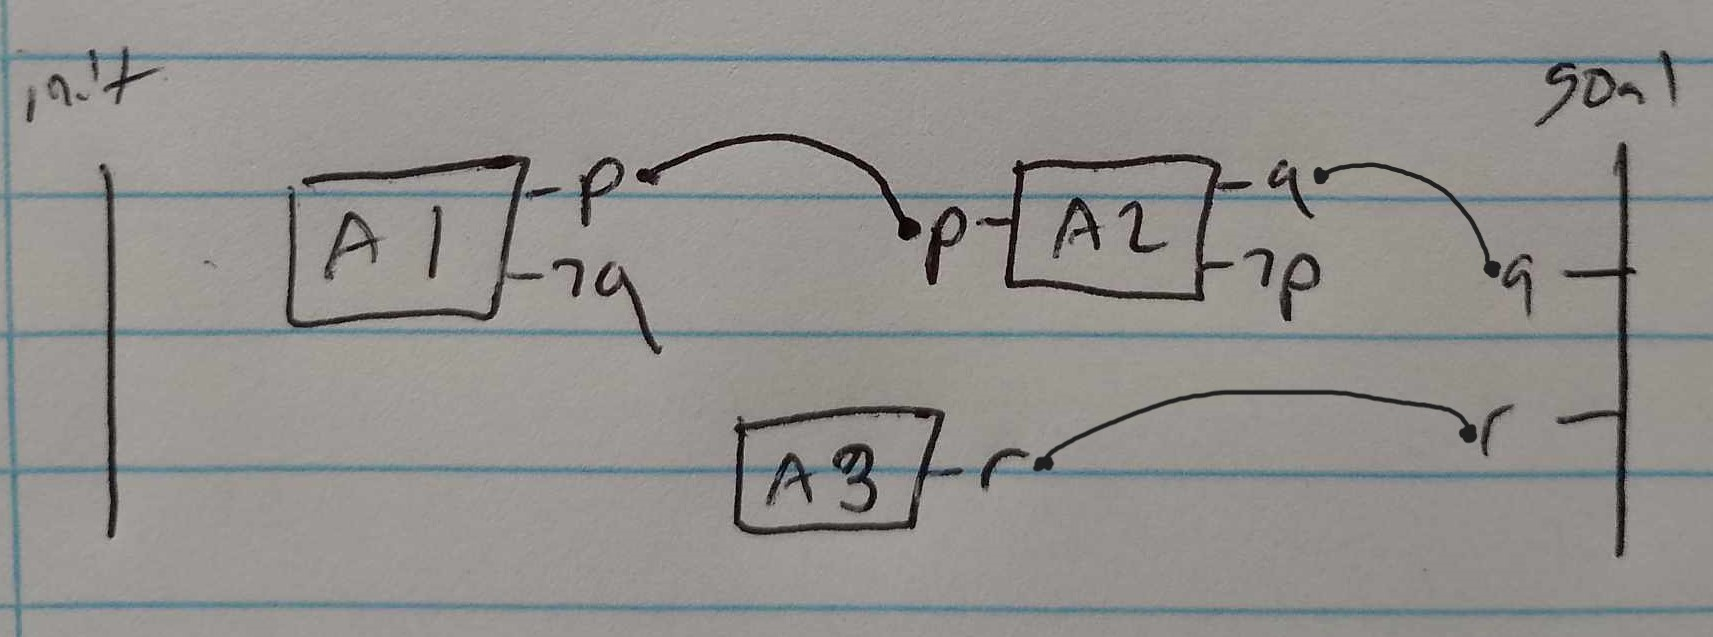
\includegraphics[width=12cm]{figures/partial_order.jpg}
    \caption{An example of a partial-order plan.\label{fig:partialOrder}}
\end{figure}


It is common knowledge that this criteria for a POCL plan is sufficient to imply that every linearization of its steps is executable, and hence a POCL plan can represent up to a factorial set of total-order solutions. However, note that the inverse is not true. There exists partial-order plans where every linearization is executable, yet there is no way to insert causal links to support every precondition without creating a causal threat, and hence there is no corresponding POCL plan. This property is explored by~\cite{Bercher2020POPvsPOCL}, including a counterexample to the inverse case in Figure 1. The paper also presents a polytime method for converting any partial-order plan where every linearization is executable into a POCL plan with the same makespan.\\


It is also well known that there is a correspondence between total-order solutions and POCL solutions to classical planning problems.

\begin{prop}
    Let $\mathcal{P}$ be a classical planning problem. There is a POCL solution to $\mathcal{P}$ if and only if there is a total-order solution to $\mathcal{P}$.
\end{prop}

The forward implication of this proposition is clear from the fact that a POCL solution represents up to a factorial number of linearizations, each of which is a valid total-order solution due to following the partial-order constraints. For example, the total-order solution in Figure~\ref{fig:totalOrder} is one possible linearization of a POCL solution shown in Figure~\ref{fig:partialOrder}. The backward direction can be done in polytime by inserting required causal links into a total-order plan to create a POCL plan which still maintains total ordering, as this is a permissible special case of partial ordering. This method is described by~\cite{Muise2016POPRelax} in Section 3.2.1.\\

In order to define POCL heuristics, we need to define a planning problem in terms of the current search node. For state-based planning this is simple to do within the framework of classical planning, as $s_I$ just needs to be updated to the current state of the search node. For POCL planning this becomes more difficult, as search nodes are partial plans containing orderings and causal links, neither of which can be easily representing within a classical planning problem. We thus define a new class of planning problems, POCL planning problems, in order to adequately represent these requirements.\\


A \textit{POCL planning problem} $\mathcal{P}$ is given by a tuple $(V, A, P_{s_I,g})$, where $V$ is a finite set of propositional variables, $A$ is a finite set of actions, and $P_{s_I,g}$ is an initial partial plan given by the tuple $(PS_I, \prec_I, CL_I)$. The partial plan $P_{s_I,g}$ must contain the two artificial actions $\mathit{init}$ and $\mathit{goal}$ as plan steps, and these actions must have defined as above according to the initial state $s_I$ and goal description $g$. Other than this requirement that $\{init, goal\}\subseteq PS_I$, $P_{s_I,g}$ can represent any partial plan. For our purposes, it will represent the partial plan at a search node within a POCL planner, for use as the initial partial plan of POCL heuristics. \\

We can now define POCL solutions to POCL planning problems. Such a solution must be a \textit{refinement} of $P_{s_I,g}$, meaning that it may only add plan steps, orderings, and causal links to $P_{s_I,g}$, but not change any of its contents. The idea of POCL search procedures which use repeated refinements, creating new POCL planning problems at each step, was introduced by~\cite{Kambhampati1997RefinementPlanning}, who named it \textit{refinement planning}.

\begin{definition}
    A partial POCL plan $P_R=(PS_R,\prec_R,CL_R)$ is called a \textit{refinement} of another partial POCL plan $P_I=(PS_I,\prec_I,CL_I)$ if and only if $PS_I\subseteq PS_R,\prec_I\subseteq \prec_R$, and $CL_I\subseteq CL_R$.
\end{definition}

\begin{definition}
    A partial POCL plan $P$ is called a \textit{POCL plan} (also \textit{POCL solution}) for a POCL planning problem $\mathcal{P}=(V, A, P_{s_I,g})$ if and only if it is a refinement of $P_{s_I,g}$, every precondition is supported by a causal link, and there are no causal threats.
\end{definition}

For our POCL heuristic, we solve the delete relaxation of a POCL plan, emulating similar heuristics for state-based planning by taking the makespan of this delete relaxation as its heuristic value. For this purpose, we now define the delete relaxation of a POCL planning problem.\\

The \textit{delete relaxation} of a POCL planning problem $\mathcal{P}=(V, A, P_{s_I,g})$ is the problem $\mathcal{P}^+$, which is $\mathcal{P}$ but with $\Del(a)=\emptyset$ for all $a\in A$, meaning that all delete effects of actions are removed. Note that the plan steps already contained within the initial plan $P_{s_I,g})$ are unaffected. Hence, only plan steps added in future refinements will have no delete effects, as they will draw from the now delete-relaxed set of actions in the POCL planning problem. This means that the implication of delete relaxation of classical planning problems, that any action which becomes executable will forever remain executable, does not hold for the delete relaxation of POCL planning problems, as a plan step from $P_{s_I,g}$ could be ordered after such an executable action, deleting one of its preconditions and making it no longer executable. This added complexity is part of the reason why solving the delete relaxation of a POCL planning problem is NP-complete, whereas in classical planning it is polytime. (TODO: in future I will probably add one or two figures visually displaying this difference, as I think it is particularly important for the reader to grasp) 

\begin{definition}
    A partial POCL plan $P$ is called a \textit{relaxed POCL plan} (also \textit{relaxed POCL solution}) for a POCL planning problem $\mathcal{P}$ if and only if $P$ is a POCL plan for $\mathcal{P^+}$.
\end{definition}


\section{Linear Programming}
\textit{Linear Programming} (LP) is a mathematical optimisation technique used to solve decision-making problems. It converts problems into many dimensional geometric shapes, where each \textit{variable} involved in the problem represents one dimension of the LP, and each \textit{constraint} of the problem is a hyperplane within that space, where one side is the region which \textit{satisfies} the constraint, and the other side is the region which doesn't. The intersection of the satisfied regions for each constraint is called the \textit{feasible region}, which is often a fully bounded shape, and represents every viable solution. The measure of optimality of a solution is represented in an LP by a directional vector, which points in the direction of better solutions. This is called the \textit{objective function}, and by finding the point in the feasible region furthest in the direction of the objective function, we can find the optimal solution to any problem able to be represented as an LP. (TODO: insert figure with a graphical representation of an LP for an example)\\

\textit{Integer Linear Programming} (ILP) is an extension of LP that allows for variables which aren't continuous, only holding integer values. It also ensures that the feasible solutions can only be integers, picking only integer valued points within the LP feasible region. This allows ILP to encode a larger range of problems, as many problems have discrete components which cannot be represented by the continuous variables in an LP. However, ILP is in a higher complexity class than LP, as integer variables make such problems much more difficult to solve and to optimise. Any ILP can be \textit{relaxed} into a corresponding LP by removing the integer restrictions on the solution and all integer variables. (TODO: insert new figure with the ILP version of the previous figure)\\

The problem of both finding a feasible solution and finding an optimal solution for LP was found to be achievable in polytime by~\cite{Khachiyan1979PolynomialLP}. However, for a polytime problem it is quite difficult to solve, and~\cite{Lawler1978LPComplexityDebate} alludes to discussion over whether solving an LP is a polytime or NP problem just a year before the first polytime algorithm was developed. In fact, the simplex algorithm, the most common algorithm before a polytime algorithm for solving LPs was found, is still the most common method for solving LPs. This is discussed by~\cite{Traub1982ComplexityOfLP}, who analyses the complexities in LP solving that allow for an NP algorithm to generally outperform a polytime one. This has meant that LP based heuristics have the potential to be quite slow compared to other polytime heuristics, especially if relaxed from ILPs such as the Lplan heuristic by~\cite{Bylander1997LplanHeuristic}. Finding feasible and optimal solutions for ILPs was shown to be NP-complete by~\cite{Karp1972ReducibilityAmongCombinatorial}. This result is more intuitive, as it is easy to see how a SAT problem, determining whether a logical boolean formula is satisfiable, can be reduced to an ILP with each boolean represented by a variable constrained to be 0 or 1.\\

Our heuristic for POCL planning, which accounts for all node information; delete effects, causal links, and orderings; has been proven to be an NP-complete problem by~\cite{Bercher2021POCLComplexities}, and so we can hence reduce this problem to an ILP in polytime. Our heuristic is concerned with finding a relaxed POCL plan for a POCL planning problem, which starts from an initial partial plan and delete relaxes the domain of actions that can be added to it. Our heuristic is designed such that any initial partial plan can be converted to an ILP problem where the optimal solution is the length of the minimum makespan of a relaxed POCL solution for the initial partial plan. An ILP based approach is particularly useful for propositional STRIPS planning, as propositional variables can be represented as 0--1 variables in an ILP, and time steps can be represented by integer values as well.\\


\section{Formalisation of LPs and ILPs}
Here we provide the formal framework for Integer Linear Programming which will be used for the remainder of this paper. We consider the problem of finding the optimal solution to Integer Linear Programming models. We first define Linear Programming, and then extend these definitions to account for integer variables and solutions.\\

A \textit{linear programming problem} $\mathcal{L}$ is given by a tuple $(V, O, C)$, where $V$ is a finite set of continuous variables, $O:V\rightarrow \mathbb{R}$ is a function which produces an \textit{objective value} $o$ from variable inputs, and $C$ is a set of linear equalities and inequalities using variables from $V$. Each variable $v\in V$ represents a changeable aspect of a problem, where any change will affect the solution/s to the problem. The objective function $O$ represents the goal of the LP and takes variables as parameters, where the goal of optimisation is to minimise the output of the objective function.  The constraints $C$ restrict the values that each variable can take, either according to constants, or in relation to the values of other variables.\\

TODO: add a mathematical example of an LP here (formally written version of the visual display of an LP from earlier).

\begin{definition}
    A set of variables $V$ is a \textit{feasible solution} to a linear programming problem if and only if all of the constraints are satisfied.
\end{definition}

\begin{definition}
    A set of variables $V$ is a \textit{optimal solution} to a linear programming problem if and only if it is the feasible solution with the minimal objective value.
\end{definition}

TODO: for the example, describe what the feasible solutions are, and what the optimal solution is\\

Linear programming is limited in its applications due to the restriction of continuous variables. Since linear programming problems are solvable in polytime, they cannot be used for our delete relaxation heuristic for POCL planning, which is NP-complete. However, since ILP is also NP-complete, and offers a convenient way to represent propositions and time steps as integers, it is relevant to our heuristic.\\

An \textit{integer linear programming problem} $\mathcal{I}$ is given by a tuple $(V, O, C)$, where $V$ is a finite set of integer-valued variables, $O:V\rightarrow \mathbb{R}$ is a function which produces an \textit{objective value} $o$ from variable inputs, and $C$ is a set of linear equalities and inequalities using variables from $V$. This is all analogous to linear programs, which the exception of $V$, which now contains integer valued variables. Note that often within the literature, ILPs are used to refer to what are more formally \textit{mixed integer linear programs} (MILPs), which combine the concepts of LPs and ILPs together to allow for both inetger-valued and continuous variables. However, in this paper we do not require such a combination, and so when we mention ILPs we specifically mean that all variables must be integer-valued.\\

TODO: add the ILP version of the LP example here

\begin{definition}
    A set of variables $V$ is a \textit{feasible solution} to an integer linear programming problem if and only if all of the constraints are satisfied and all variables are integer valued.
\end{definition}

\begin{definition}
    A set of variables $V$ is a \textit{optimal solution} to an integer linear programming problem if and only if it is the feasible solution with the minimal objective value.
\end{definition}

TODO: for the example, describe feasible and optimal solutions.\\

While an ILP represents a single problem, often we want to use ILP to solve a class of problems. This requires a transformation which takes a set of problem parameters that define a specific instance of the problem class, and produces an ILP problem from them. This is called an \textit{ILP model}, and is formally defined as a transformation $\mathcal{M}:X\rightarrow \mathcal{I}$, where $X$ is a set of parameters which can vary in type, and $\mathcal{I}$ is an ILP problem. An example of a problem class for which an ILP model would be useful is sudokus, where the given digits in a specific sodoku puzzle would be the parameters for the ILP model used to generate an ILP problem which represents that soduku puzzle. We use an ILP model to define our heuristics, as when solving a relaxed POCL planning problem, the POCL planning problem represents the parameters $X$, which our model translates into an ILP problem.\\

Another useful concept in ILP is \textit{LP relaxation}. An LP relaxation of an ILP problem is a corresponding LP problem where variables are no longer restricted to being integer-valued, and become continuous. LP relaxations are very useful ways of finding simple relaxations to NP-hard problems, as any problem that can be represented as an ILP problem can very easily be relaxed into an LP problem. 